
\section{Modelo CNC} 

\begin{frame}
\frametitle{Clasificador Neuronal Competitivo}
\graphictoccnc
\end{frame}

\subsection{Redes Competitivas}
\begin{myframe}\frametitle{Redes neuronales competitivas}
\begin{columns}
\begin{column}{0.5\textwidth}
\centering
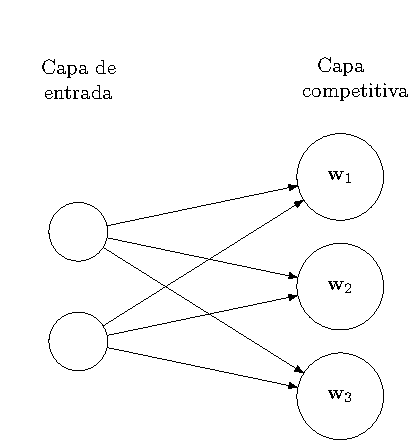
\includegraphics[width=\textwidth]{aprendizaje/cpn} 
\end{column}
\begin{column}{0.5\textwidth}
\includegraphics<1>[width=\textwidth]{aprendizaje/cpn_clustering1} 
\includegraphics<2>[width=\textwidth]{aprendizaje/cpn_clustering2} 
\includegraphics<3>[width=\textwidth]{aprendizaje/cpn_clustering3} 
\centering
\end{column}
\end{columns}
\blockitemize{Características}{
\item Clustering, no clasificación
\item Modelo base del CNC
}
\end{myframe}

\begin{myframe}\frametitle{Funcionamiento: Clustering}
\centering

\begin{columns}
\begin{column}{0.5\textwidth}
\centering
\foreach \x in {1,2,3,4} {
  \includegraphics<\x>[width=\textwidth]{aprendizaje/cpn_funcionamiento_\x} 
}
\end{column}
\begin{column}{0.5\textwidth}
\foreach \x in {1,2,3,4} {
  \includegraphics<\x>[width=\textwidth]{aprendizaje/cpn_funcionamiento_geometria_\x} 
}
\centering
\end{column}
\end{columns}
%\blockitemize{Regla de activación}{ 
%  \item Neurona $2$ ganó: $d( \wv_2,\xv) < d(\wv_1,\xv)$ y $d( \wv_2,\xv) < d(\wv_3,\xv)$
%  \item Neurona $j$ es ganadora si $d( \wv_j,\xv) < d(\wv_i,\xv), \; i \neq j$
%}
\end{myframe}


\begin{frame}
\frametitle{Entrenamiento (de a uno)}
\centering

\foreach \x in {1,2,3,4,5,6,7,8,9,10} {
  \includegraphics<\x>[width=0.8\textwidth]{aprendizaje/cpn_entrenamiento_neurona_\x} 
}

%\blockitemize{Regla de actualización}{
%\item Dado un $\xv$, supongamos que la neurona $j$ es ganadora
%\item $\wv_j := \wv_j + \alpha (-\wv_j + \xv)$
%}

\end{frame}


\begin{frame}
\frametitle{Entrenamiento (Todos los ejemplares)}
\centering

\foreach \x in {1,2,3,4,5} {
  \includegraphics<\x>[width=0.8\textwidth]{aprendizaje/cpn_entrenamiento_\x} 
}

%\blockitemize{Regla de actualización}{
%\item Dado un $\xv$, supongamos que la neurona $j$ es ganadora
%\item $\wv_j := \wv_j + \alpha (-\wv_j + \xv)$
%\item \textbf{Repetir con todos los ejemplares hasta convergencia}
%}
\end{frame}


  
\subsection{Clasificador neuronal competitivo (CNC)}

\begin{frame}
\frametitle{Clasificador neuronal competitivo (CNC)}

    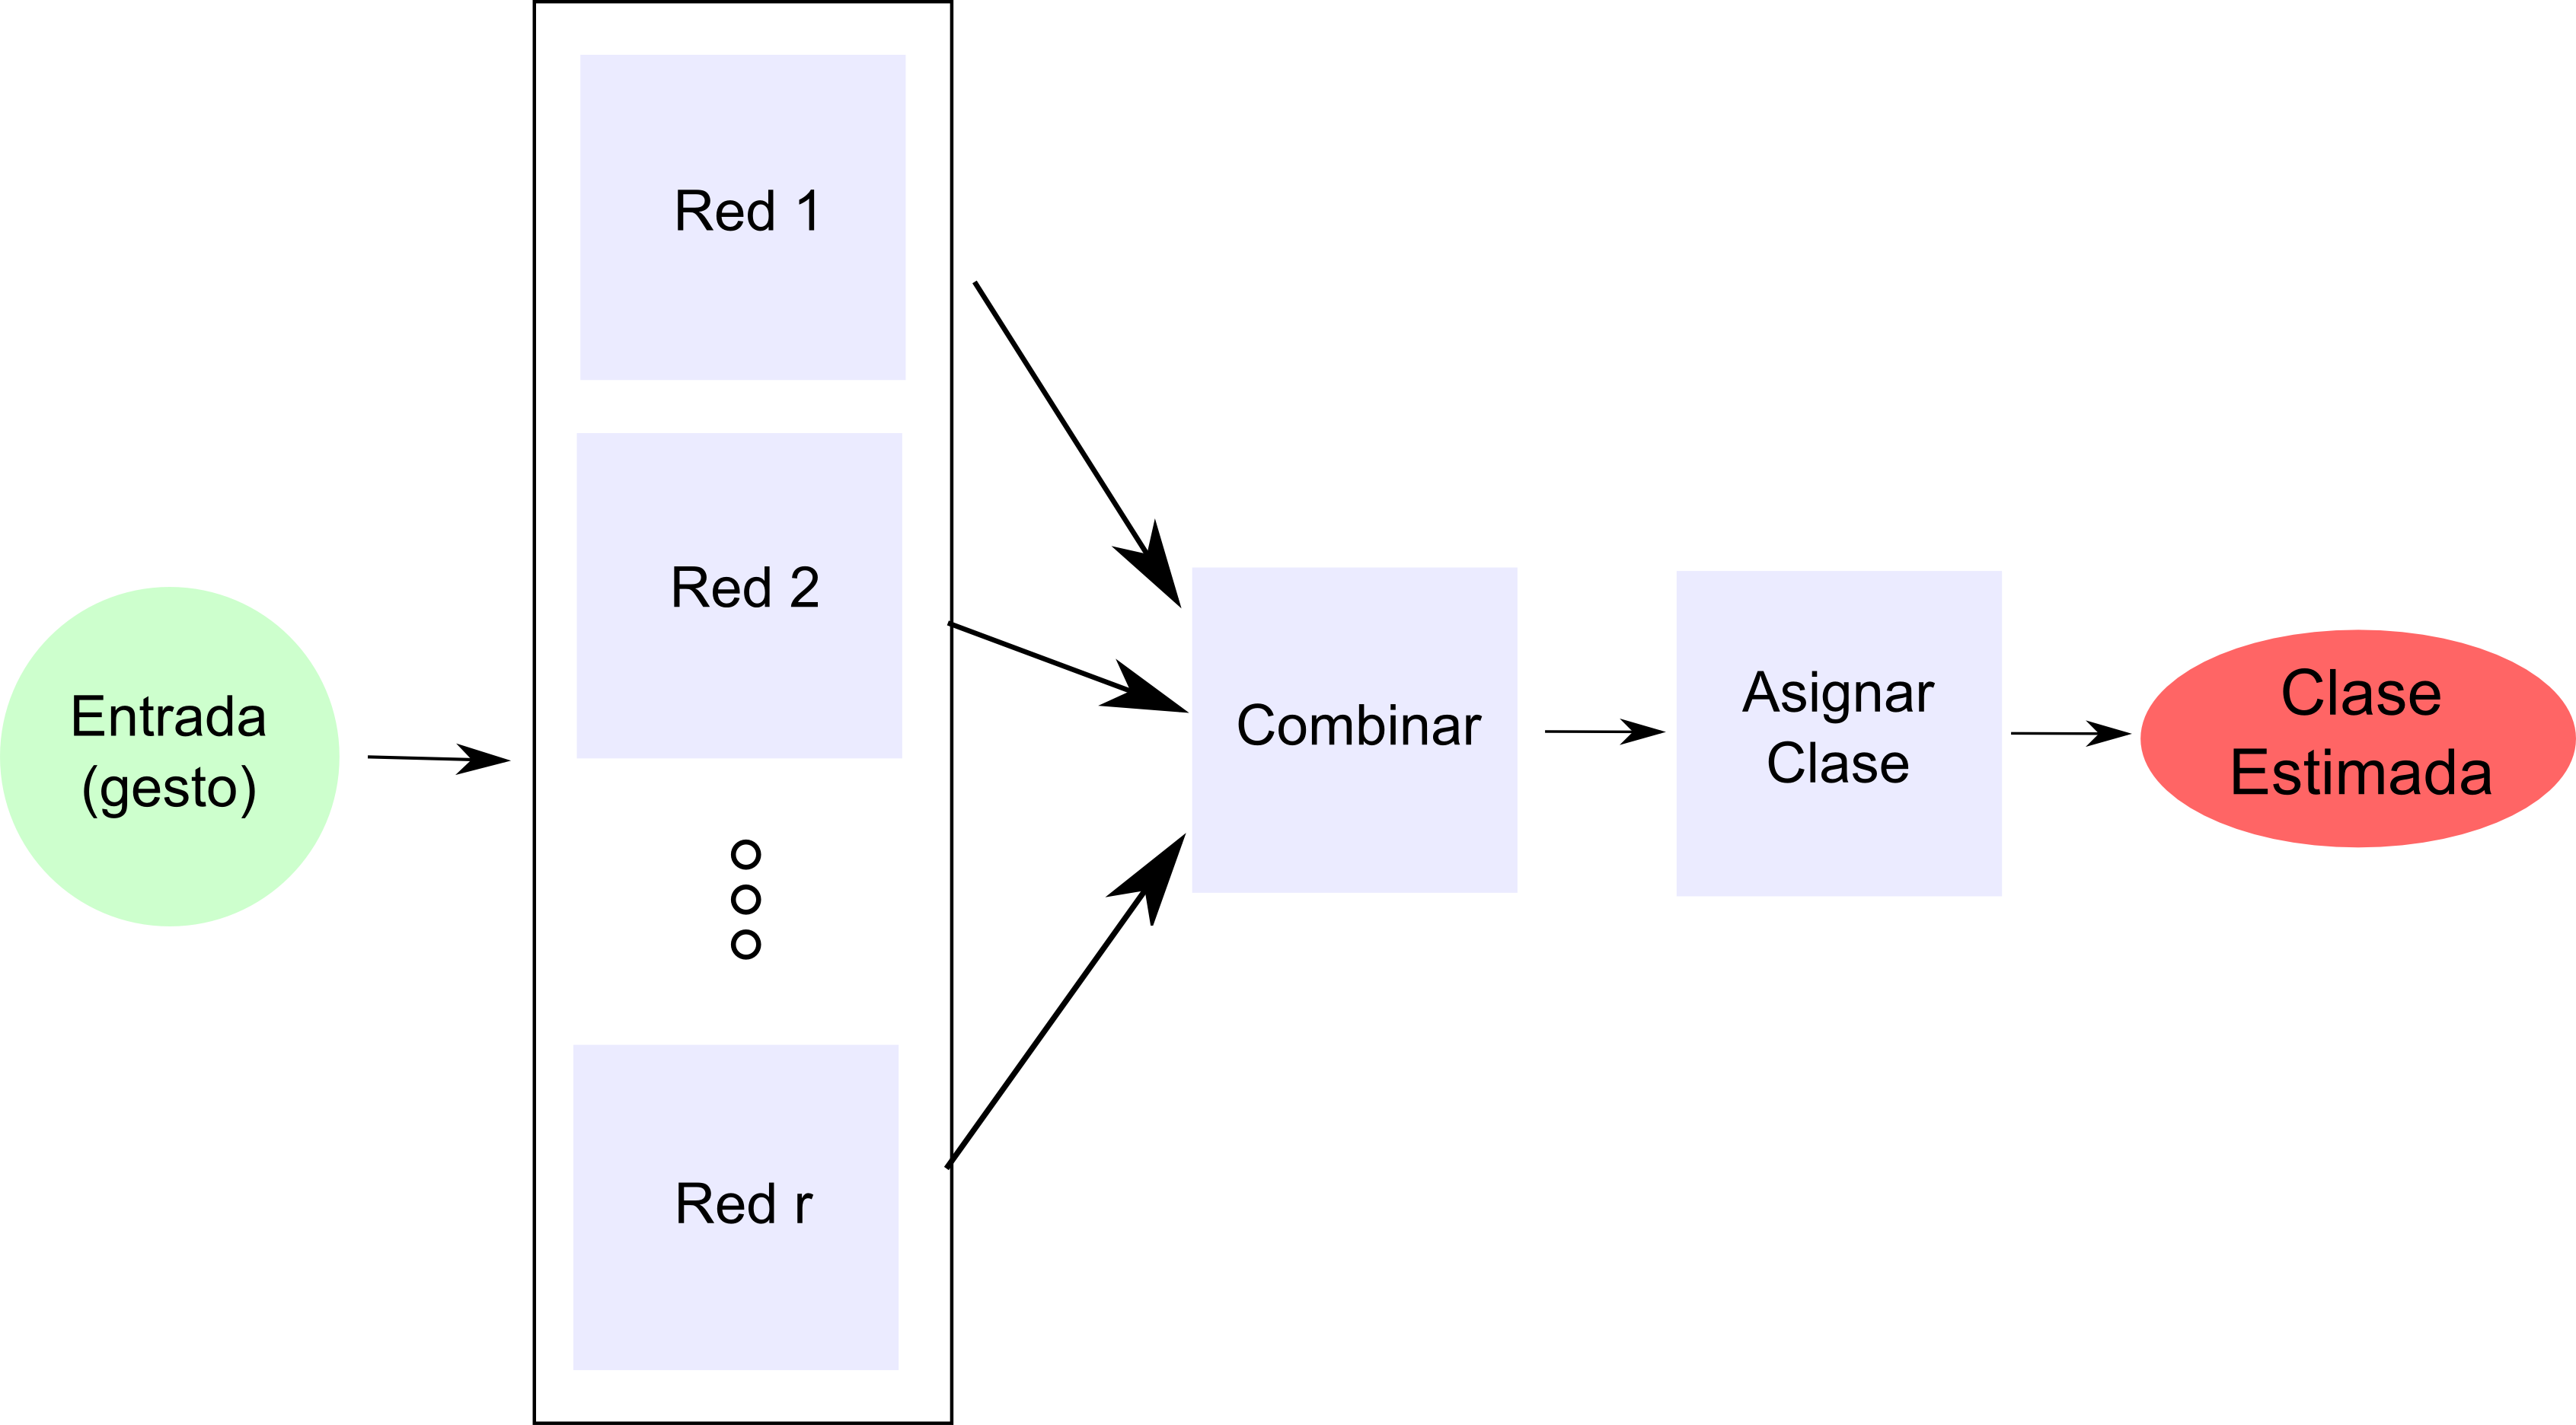
\includegraphics[width=0.85\linewidth]{cnc/bagging}
\begin{columns}
    \begin{column}{0.5\textwidth}
      \begin{itemize}
        \item Basado en redes neuronales competitivas
        \item Buen rendimiento aún con pocos gestos para entrenar
      \end{itemize}
    \end{column}
    \begin{column}{0.5\textwidth}
          \begin{itemize}
            \item Esquema de \textbf{bagging}
            \item Puede usarse sin re-muestrear los gestos.
          \end{itemize}
    \end{column}
  \end{columns}
\end{frame}



\subsection{CNC: Funcionamiento de cada red}

\begin{myframe}
\frametitle{Idea: Descartar secuencia de direcciones }
\centering
\includegraphics[scale=0.8]{cnc/bolsadirecciones_angosto}
\end{myframe}

\begin{myframe}
\frametitle{Estructura de cada red}
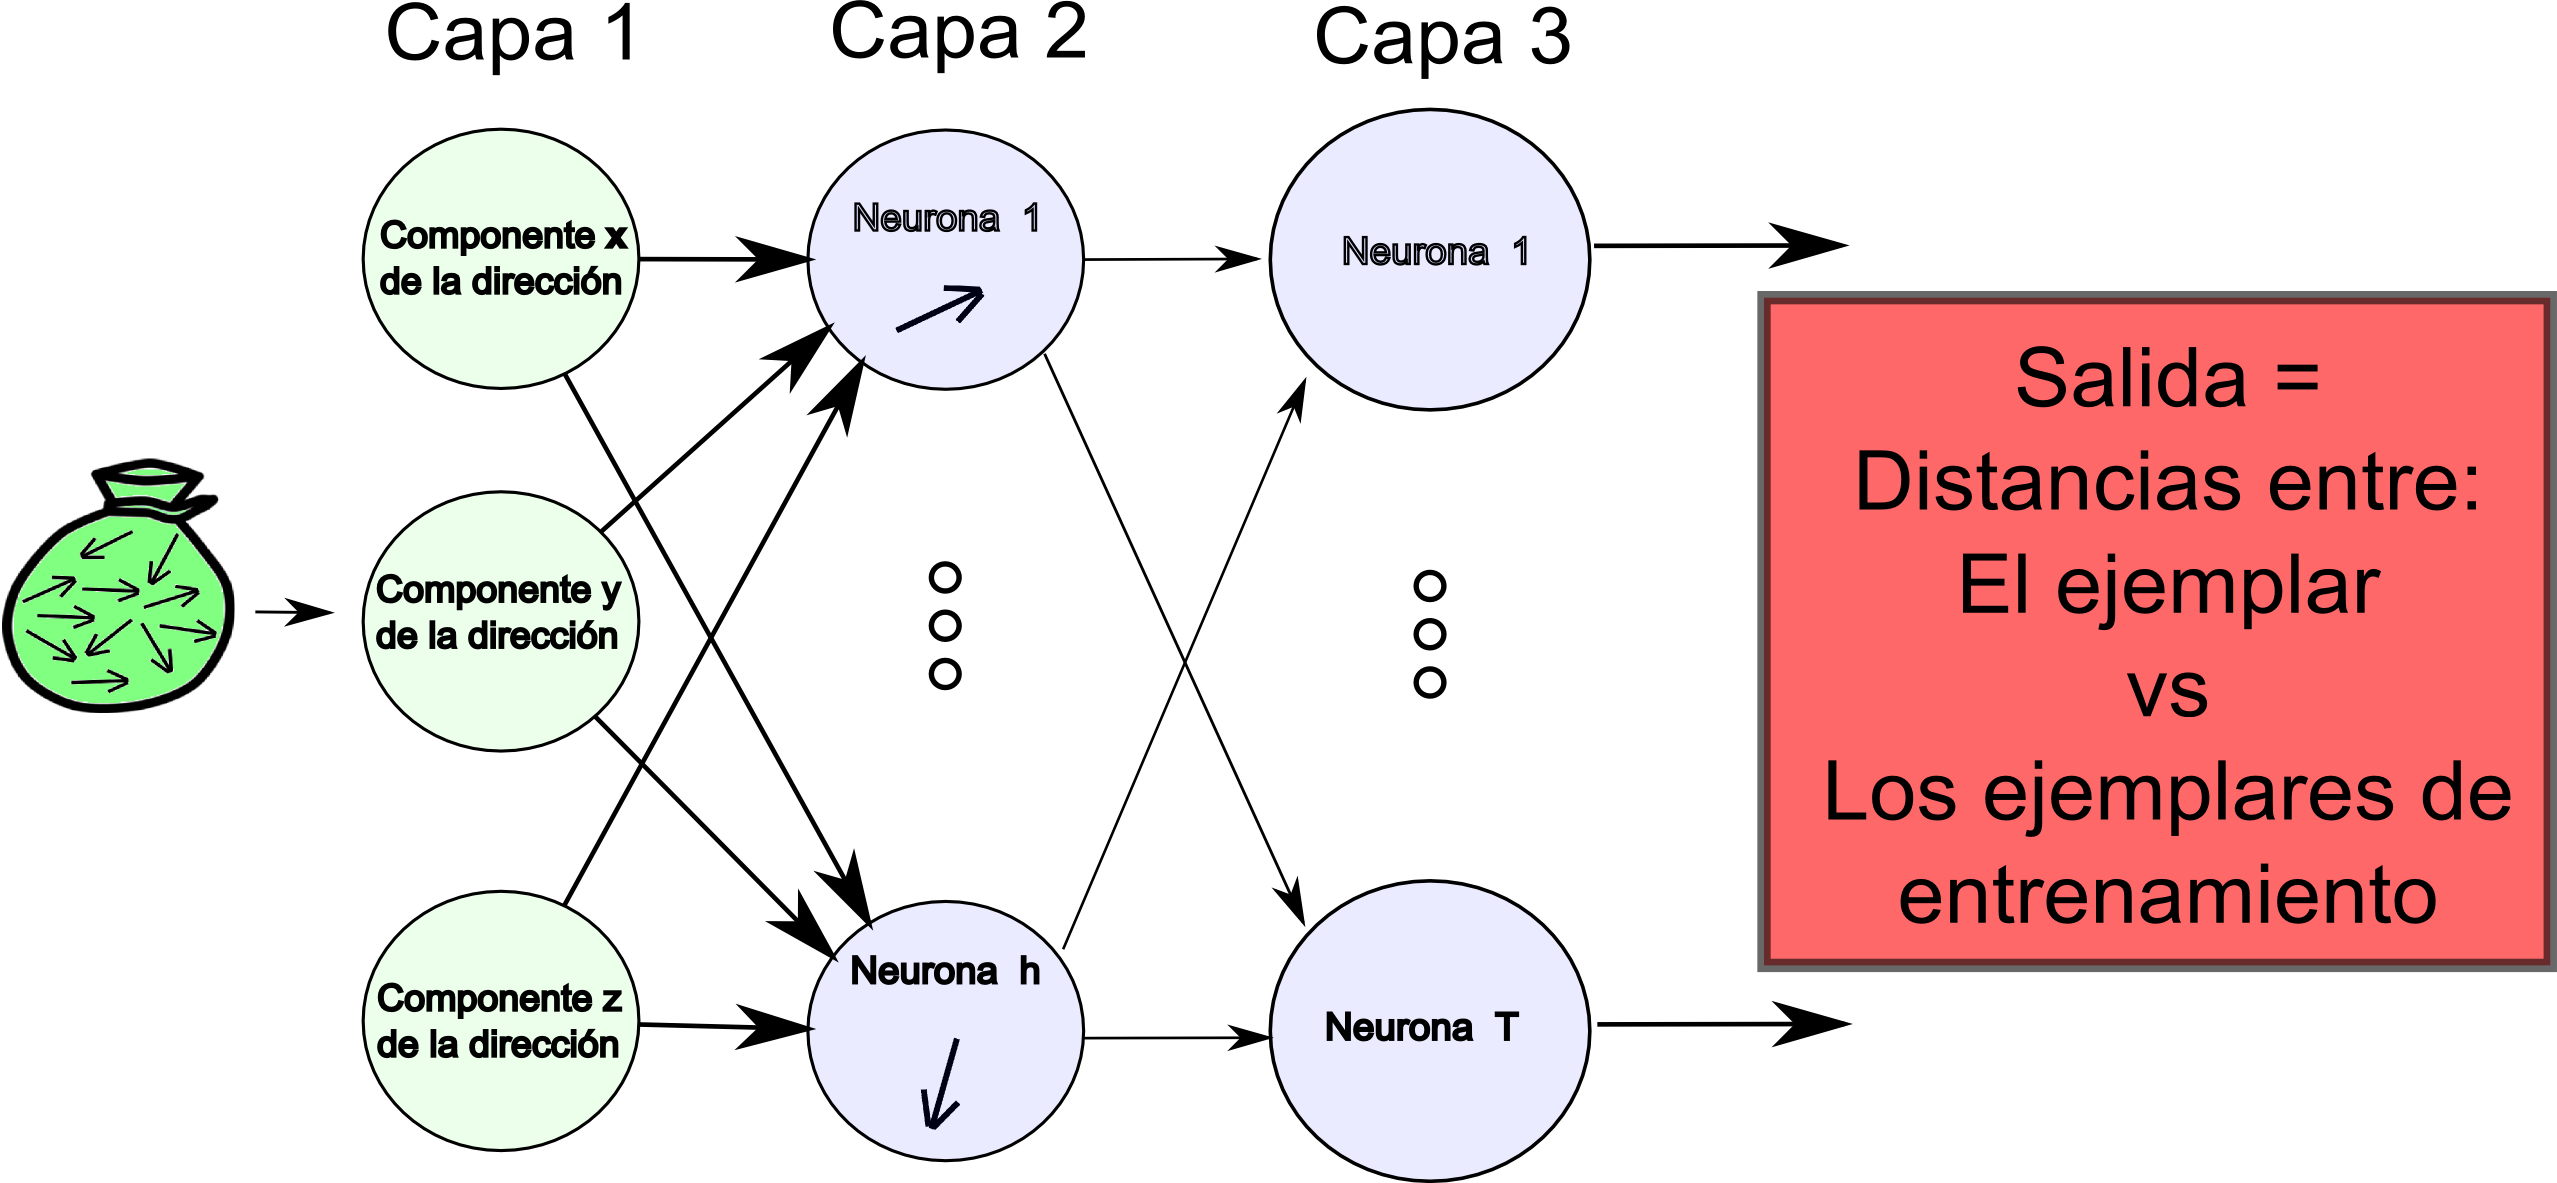
\includegraphics[width=\textwidth]{cnc/estructura_basica}

\blockitemize{}{
\item $h=$ Cantidad de neuronas de la capa 2, $\rightarrow$ parámetro a seleccionar
\item $T=$ Cantidad de gestos del conjunto de entrenamiento

}
\end{myframe}


\begin{myframe}
\frametitle{Idea: Clustering de direcciones}
\centering
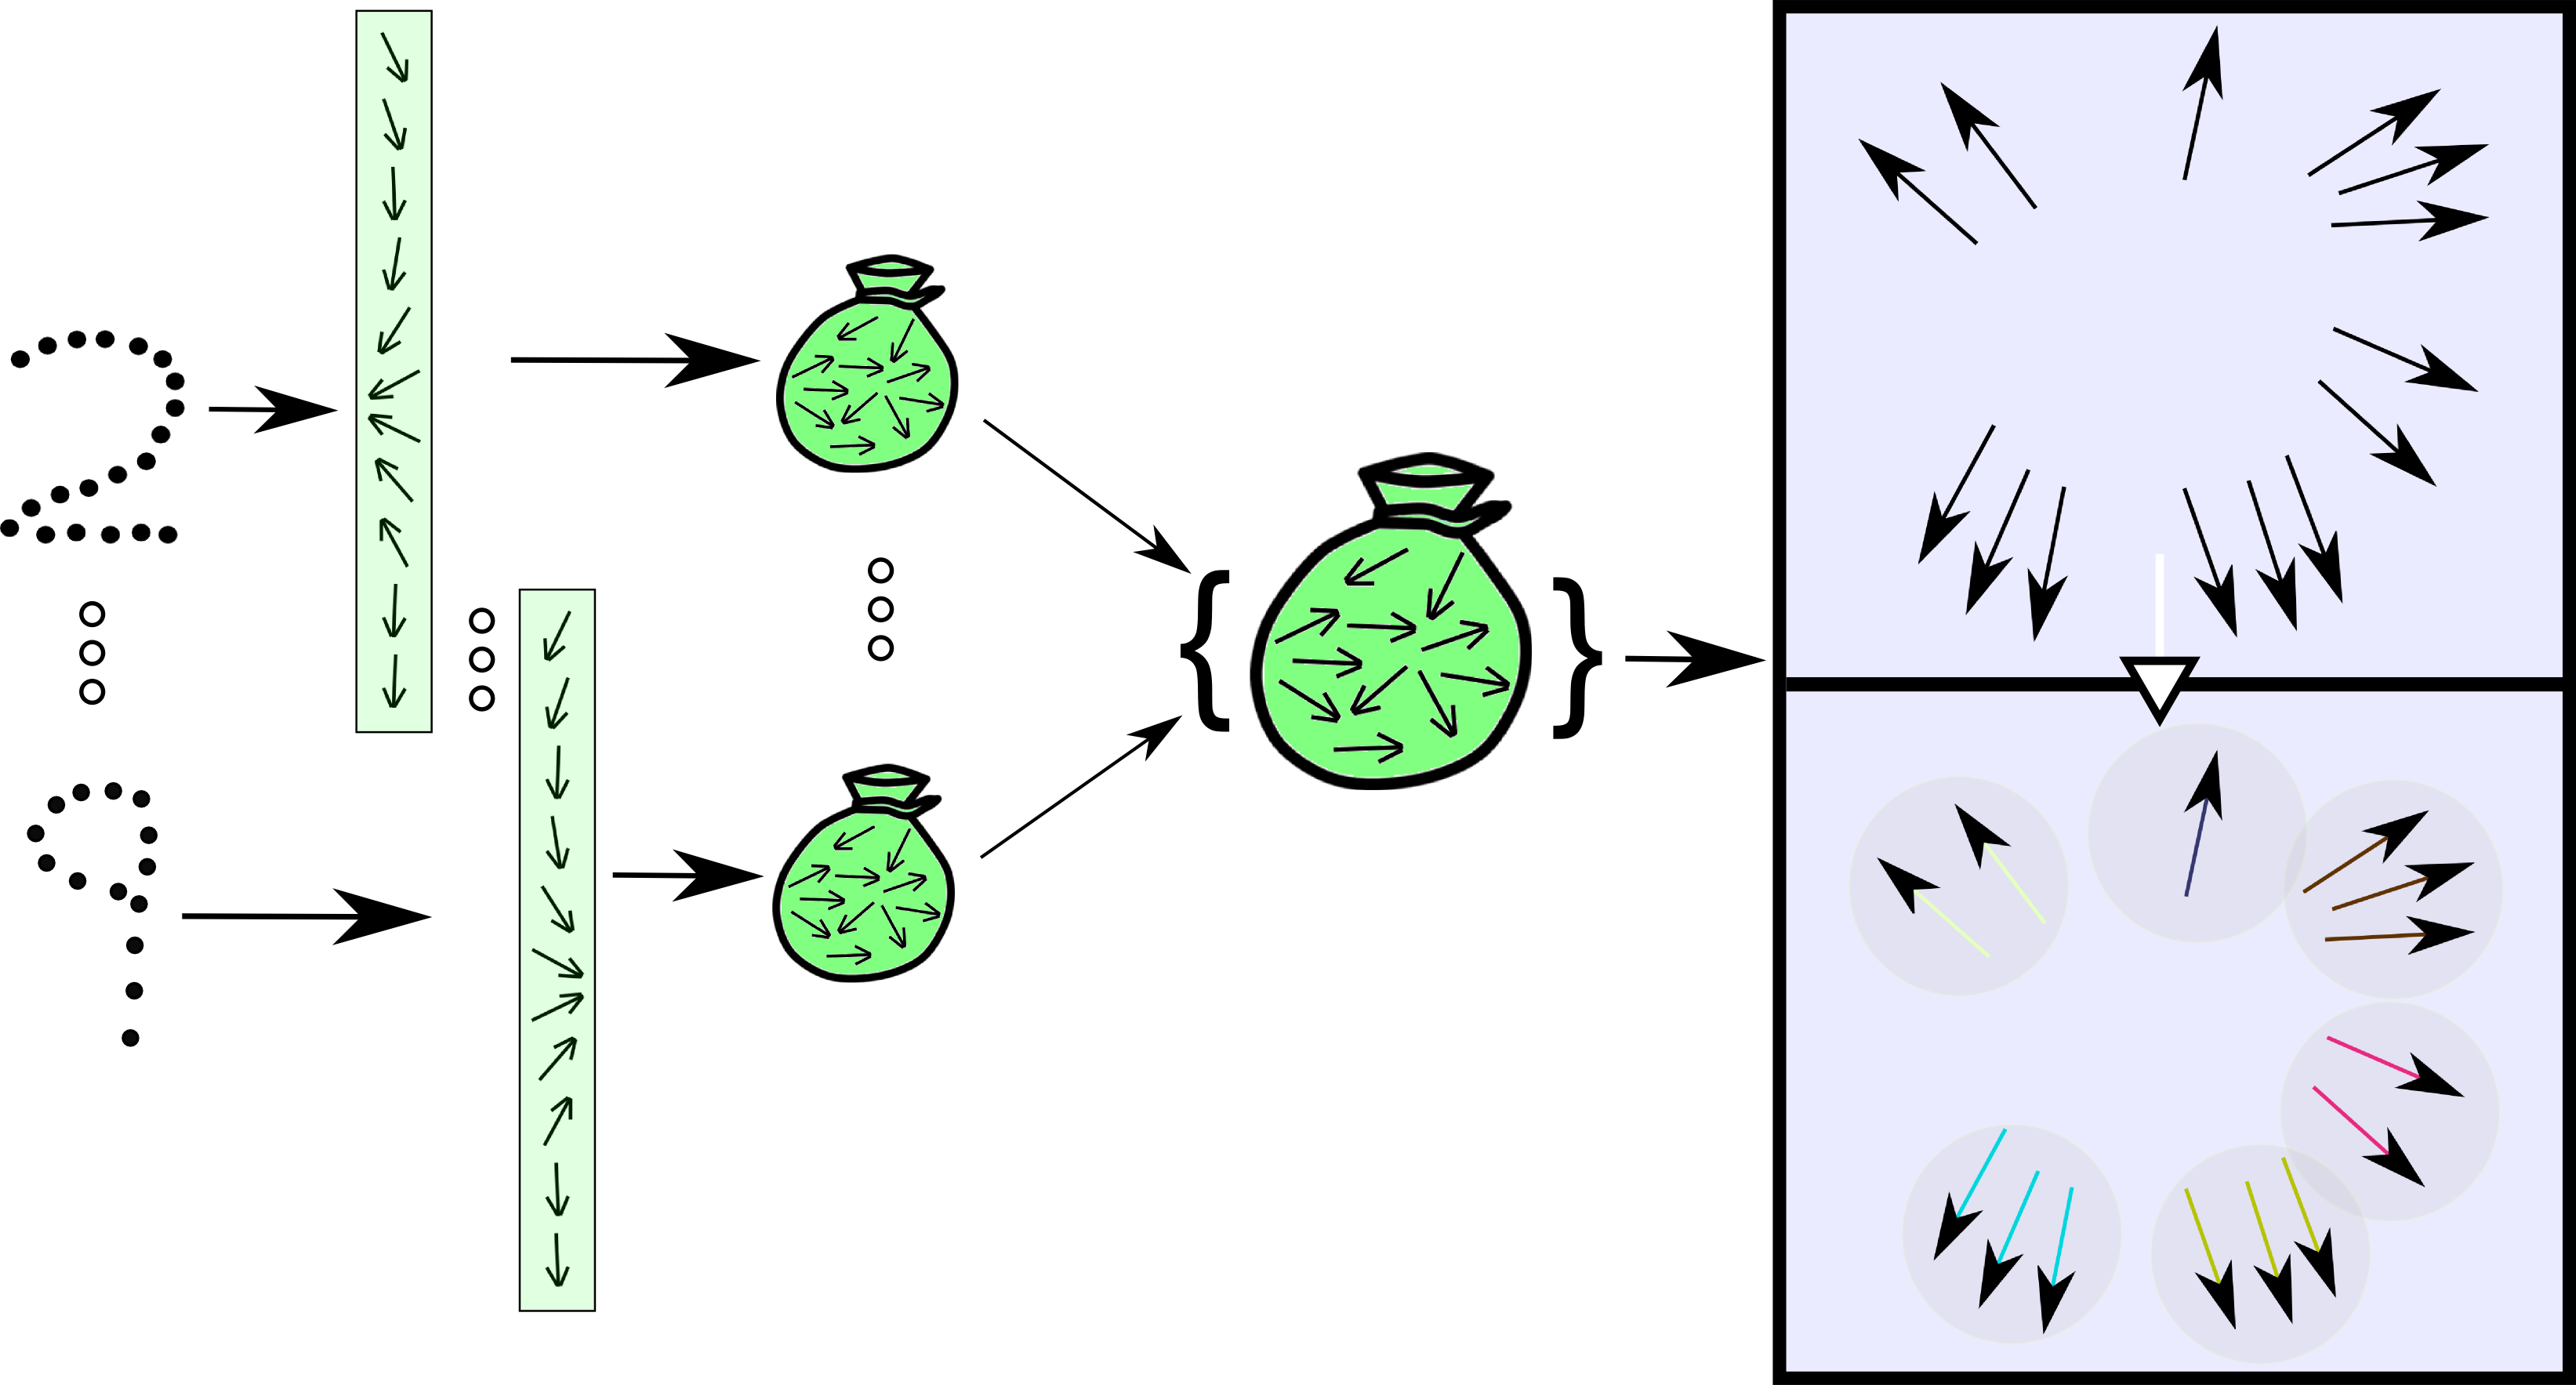
\includegraphics[scale=0.5]{cnc/bolsadireccionestodoslosgestos_angosto}
\blockitemize{}{
\item $h=$ Cantidad de neuronas de la capa 2, $\rightarrow$ parámetro a seleccionar
}
\end{myframe}

\begin{myframe}
\frametitle{Entrenamiento capa 2}
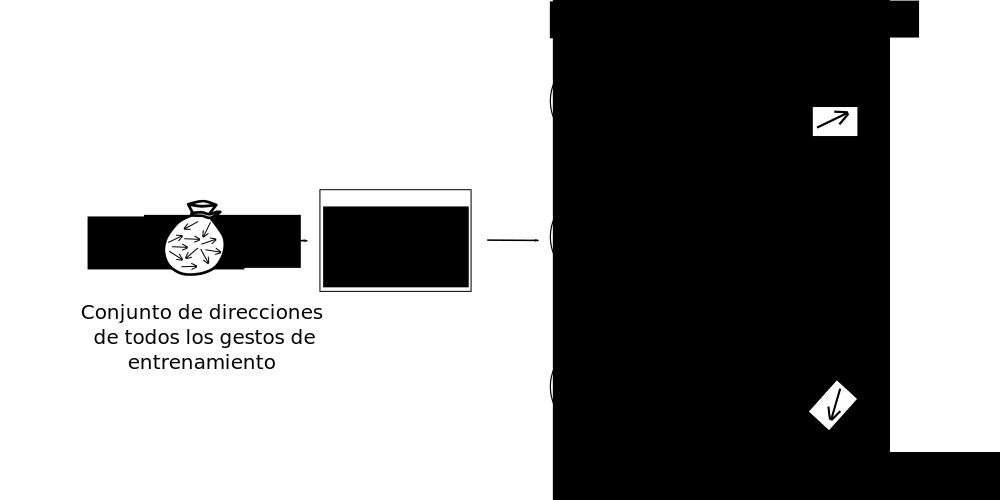
\includegraphics[width=\textwidth]{cnc/capa1}
\end{myframe}


\begin{myframe}
\frametitle{Idea: Codificación de gestos: Ejemplo}
\centering

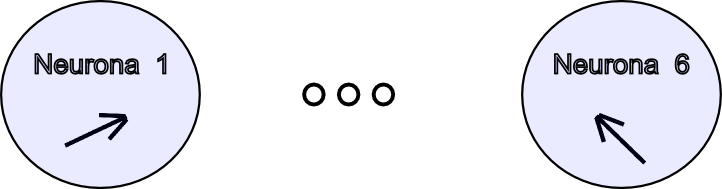
\includegraphics[scale=1]{cnc/neuronas_capa1}\\
\vspace{10pt}
\includegraphics<1>[scale=0.5]{cnc/codificacion1}
\includegraphics<2>[scale=0.5]{cnc/codificacion2}
\includegraphics<3>[scale=0.5]{cnc/codificacion3}
\end{myframe}

\begin{myframe}
\frametitle{Entrenamiento capa 3}
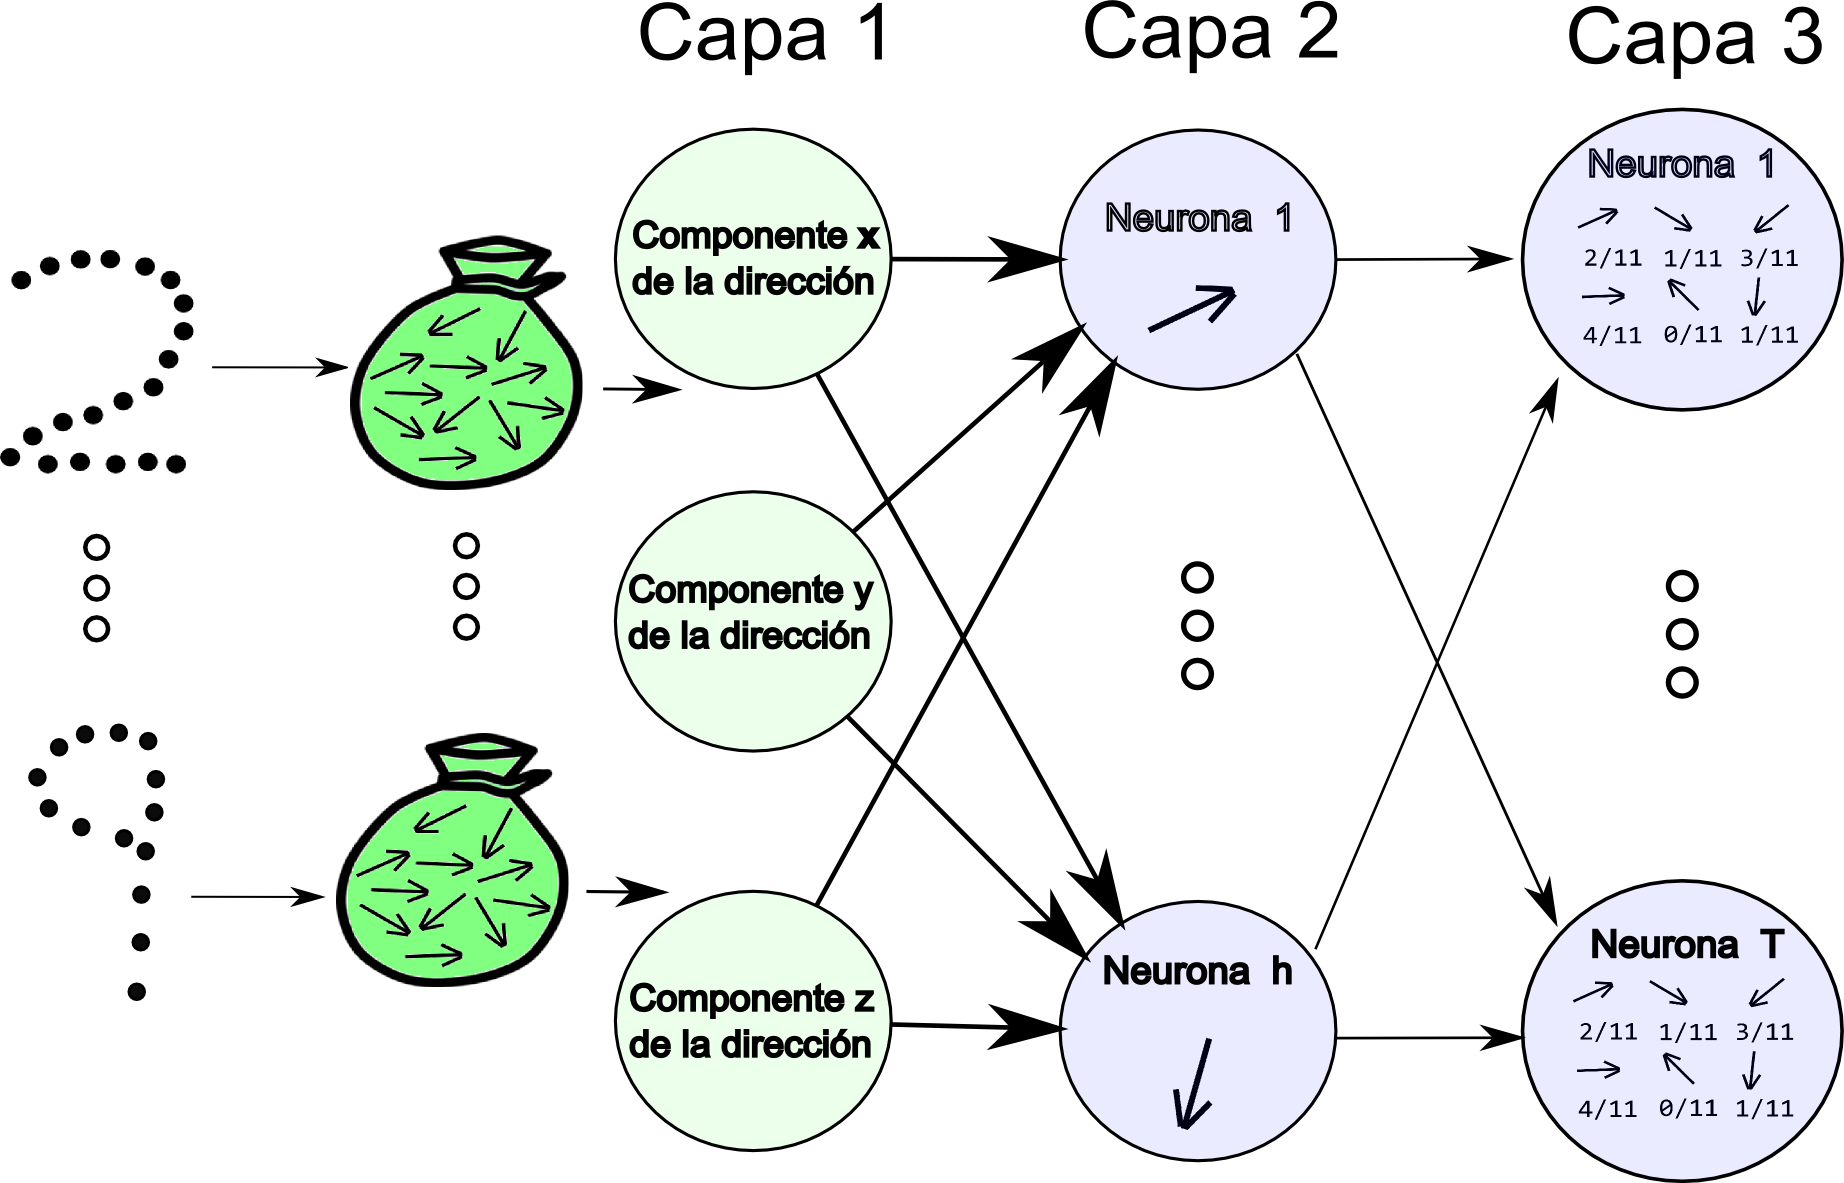
\includegraphics[width=\textwidth]{cnc/capa2_entrenamiento}
\end{myframe}



\begin{myframe}
\frametitle{Idea: Asignación de clase a un gesto nuevo}
\centering

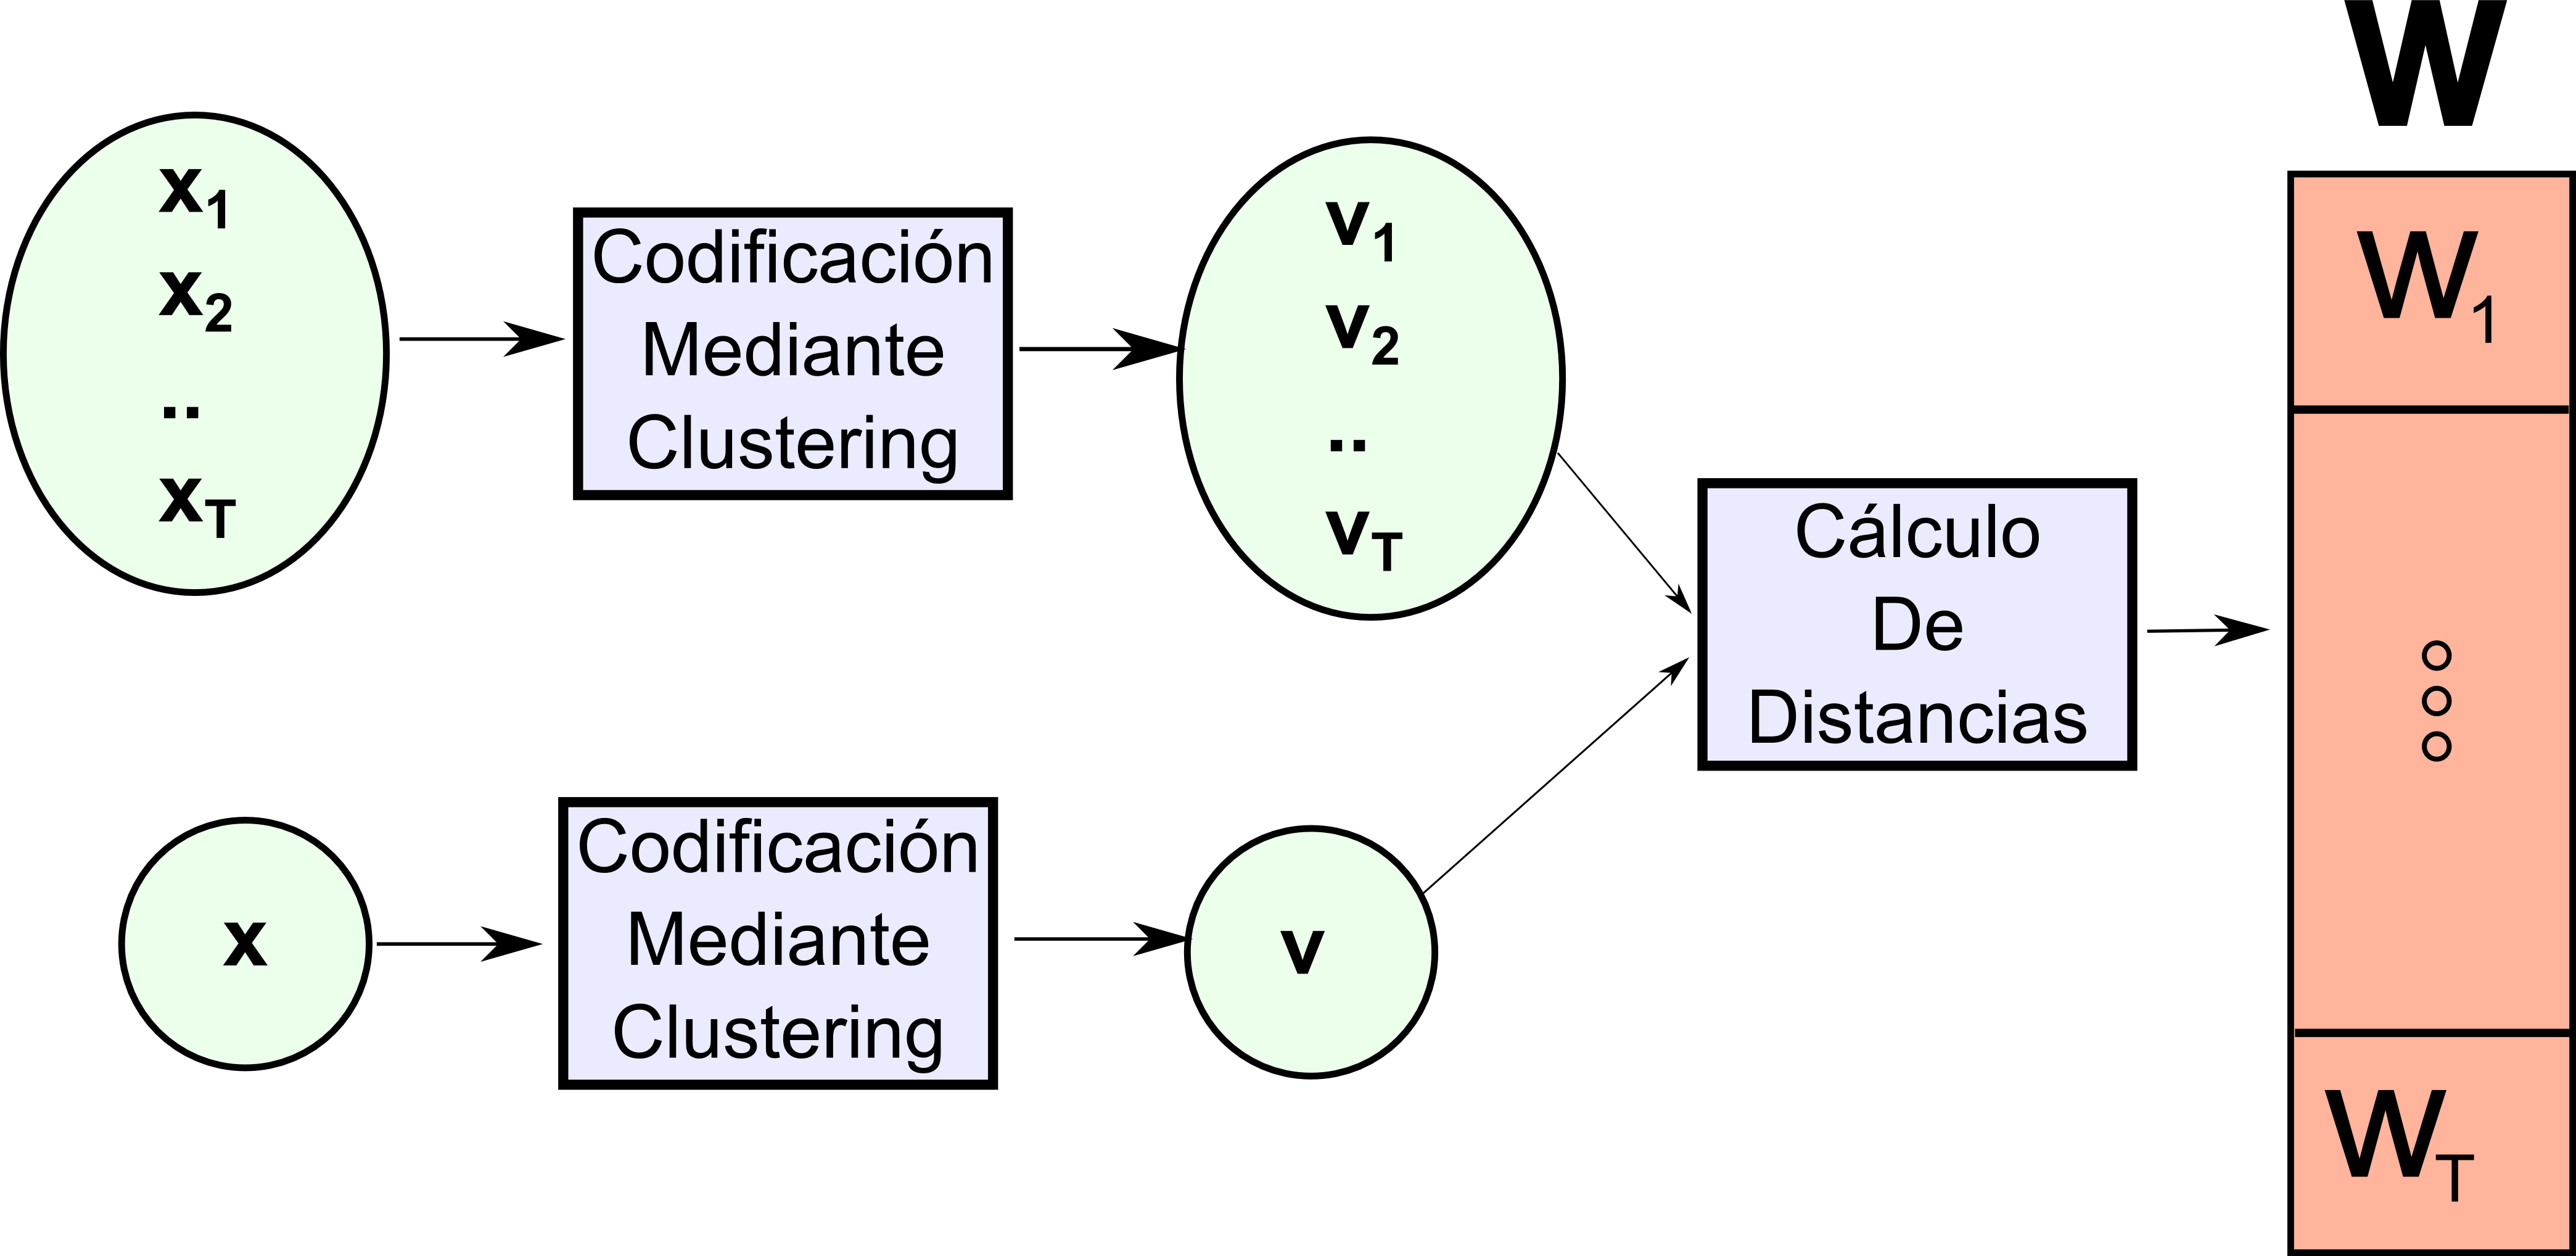
\includegraphics[scale=0.33]{cnc/clasificacion}\\
\blockitemize{}{
\item $T=$ Cantidad de gestos del conjunto de entrenamiento
\item \textbf{W} = Vector de distancias entre $\ve{v}$ y $\ve{v}_i$, $i=1,\dots,T$
}
\end{myframe}


\begin{myframe}
\frametitle{Funcionamiento capa 2}
\includegraphics[width=\textwidth]{cnc/capa1_funcionamiento}
\end{myframe}

\begin{myframe}
\frametitle{Funcionamiento capa 3}
\includegraphics[width=0.9\textwidth]{cnc/capa2_funcionamiento}
\end{myframe}


\begin{myframe}
\frametitle{Estructura Final de cada red}
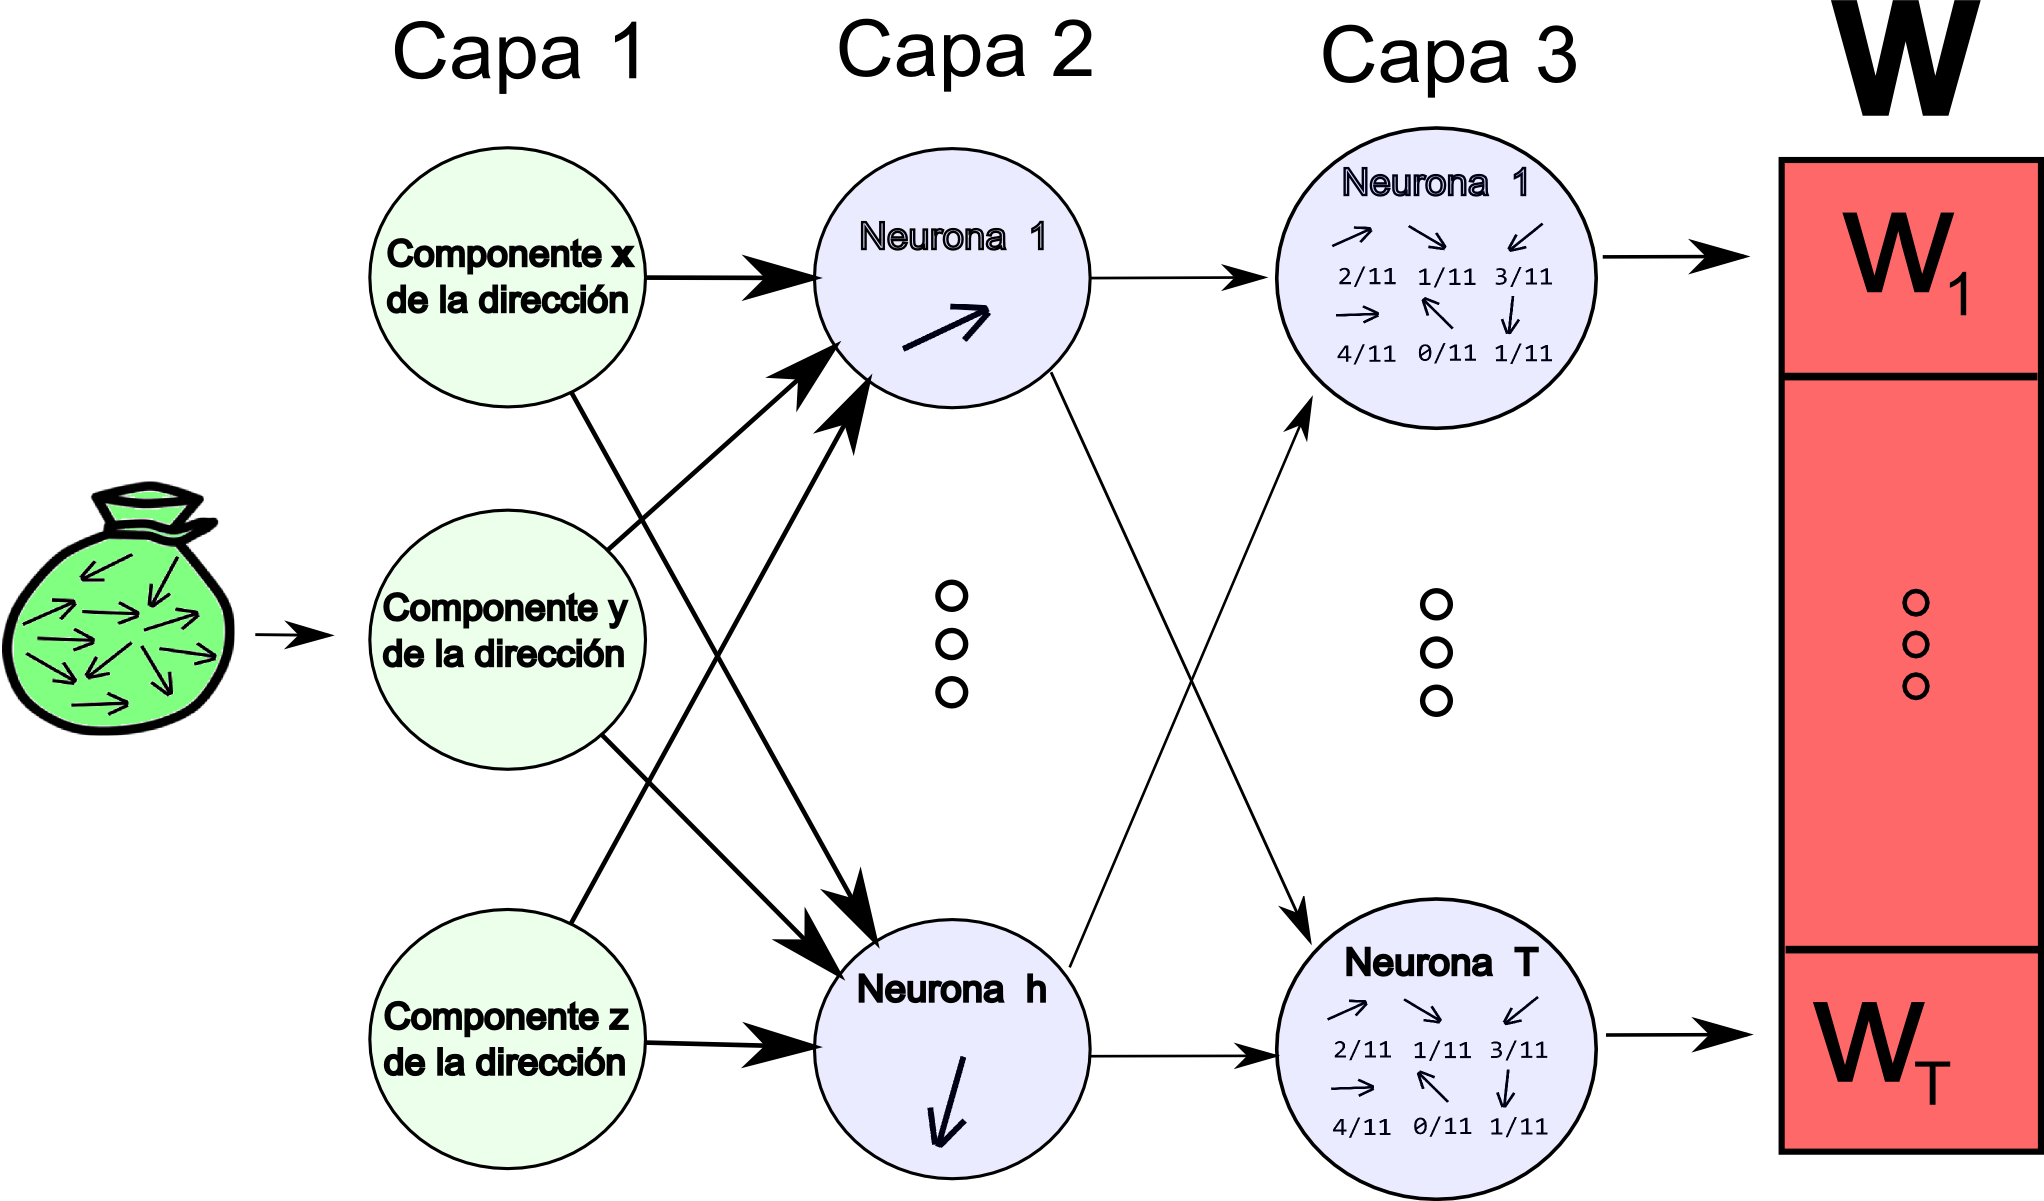
\includegraphics[width=\textwidth]{cnc/estructura}
\end{myframe}

\subsection{Bagging}

\begin{myframe}
\frametitle{Bagging}
\centering
\small

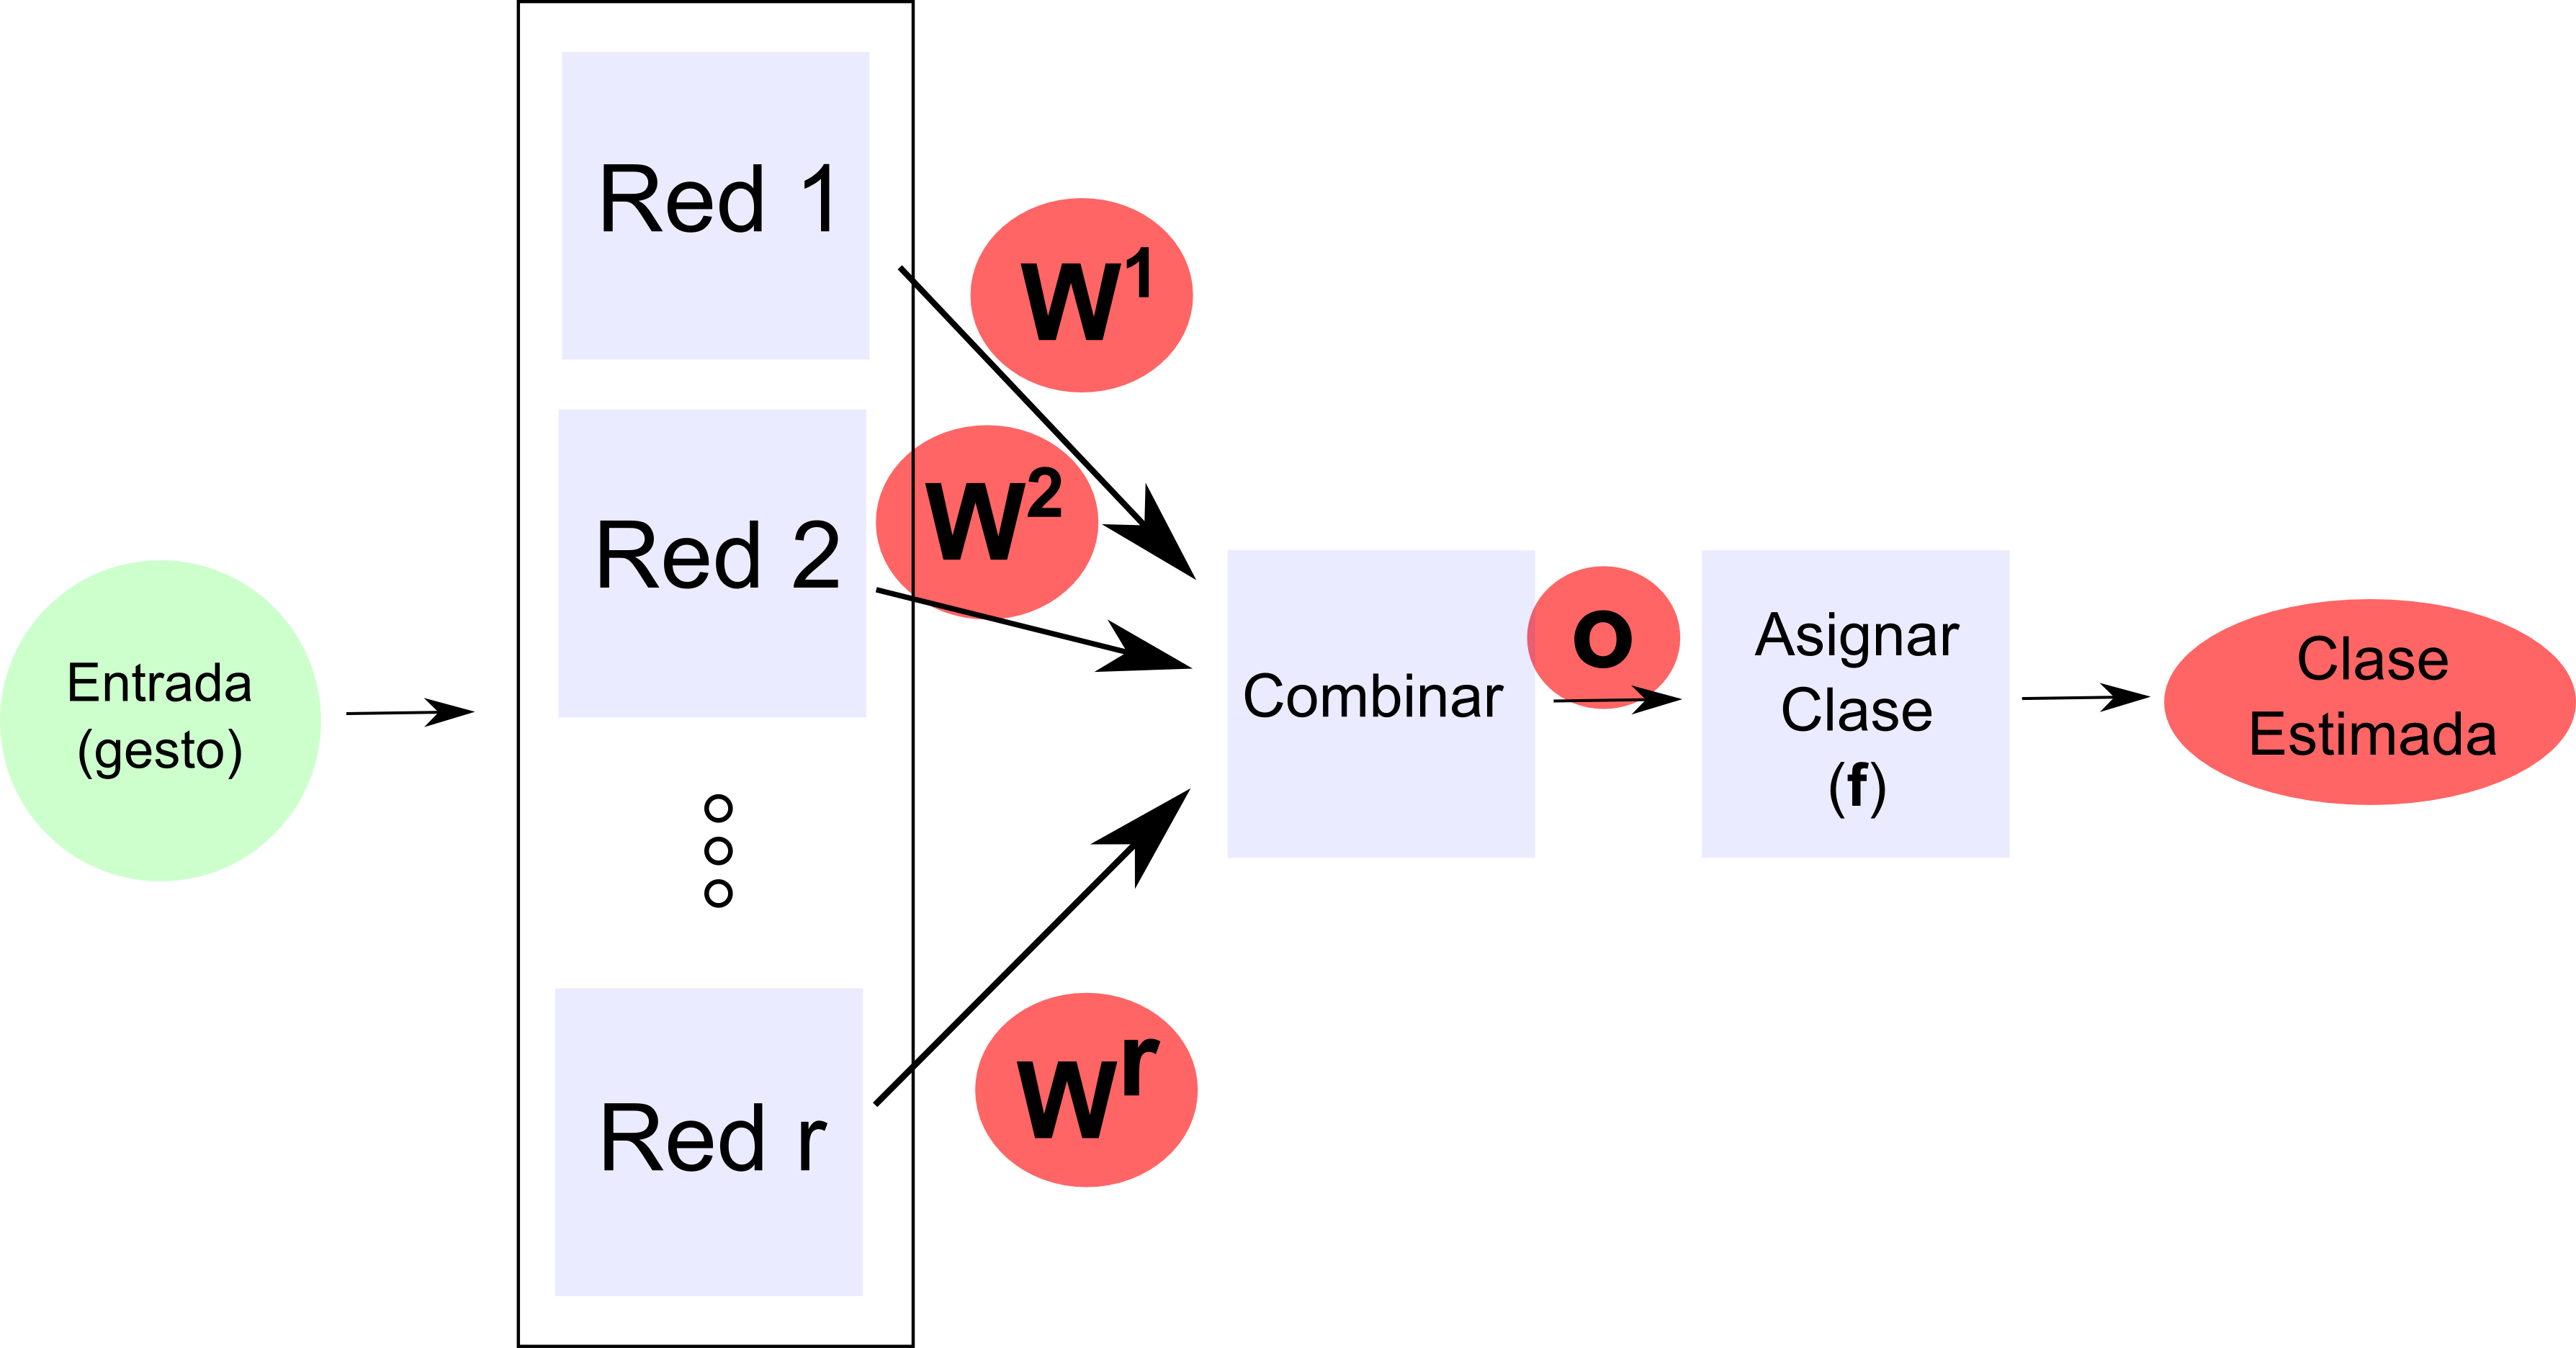
\includegraphics[width=0.7\textwidth]{cnc/output}
\begin{block}{Salida del clasificador para un gesto $\ve{x}$}

\begin{columns}
\centering
\begin{column}{0.23\linewidth}
\centering
$o = \frac{\sum\limits_{i=1}^{r} \ve{W}^i}{r}$ 
\end{column}

\begin{column}{0.37\linewidth}
\centering
$k = \min\limits_j o_j, \, j=1,\dots,T$ 
%$\rightarrow$ k = Índice del gesto de entrenamiento con menor distancia a $\ve{x}$   
\end{column}

\begin{column}{0.23\linewidth}
\centering
$f(\ve{x})= clase(k)$\\
%$\rightarrow$ f= Clase del gesto $k$
\end{column}

\end{columns}

\end{block}

\end{myframe}

\subsection{CNC*}

\begin{myframe}
\frametitle{CNC* = CNC sin re-muestrear los gestos}
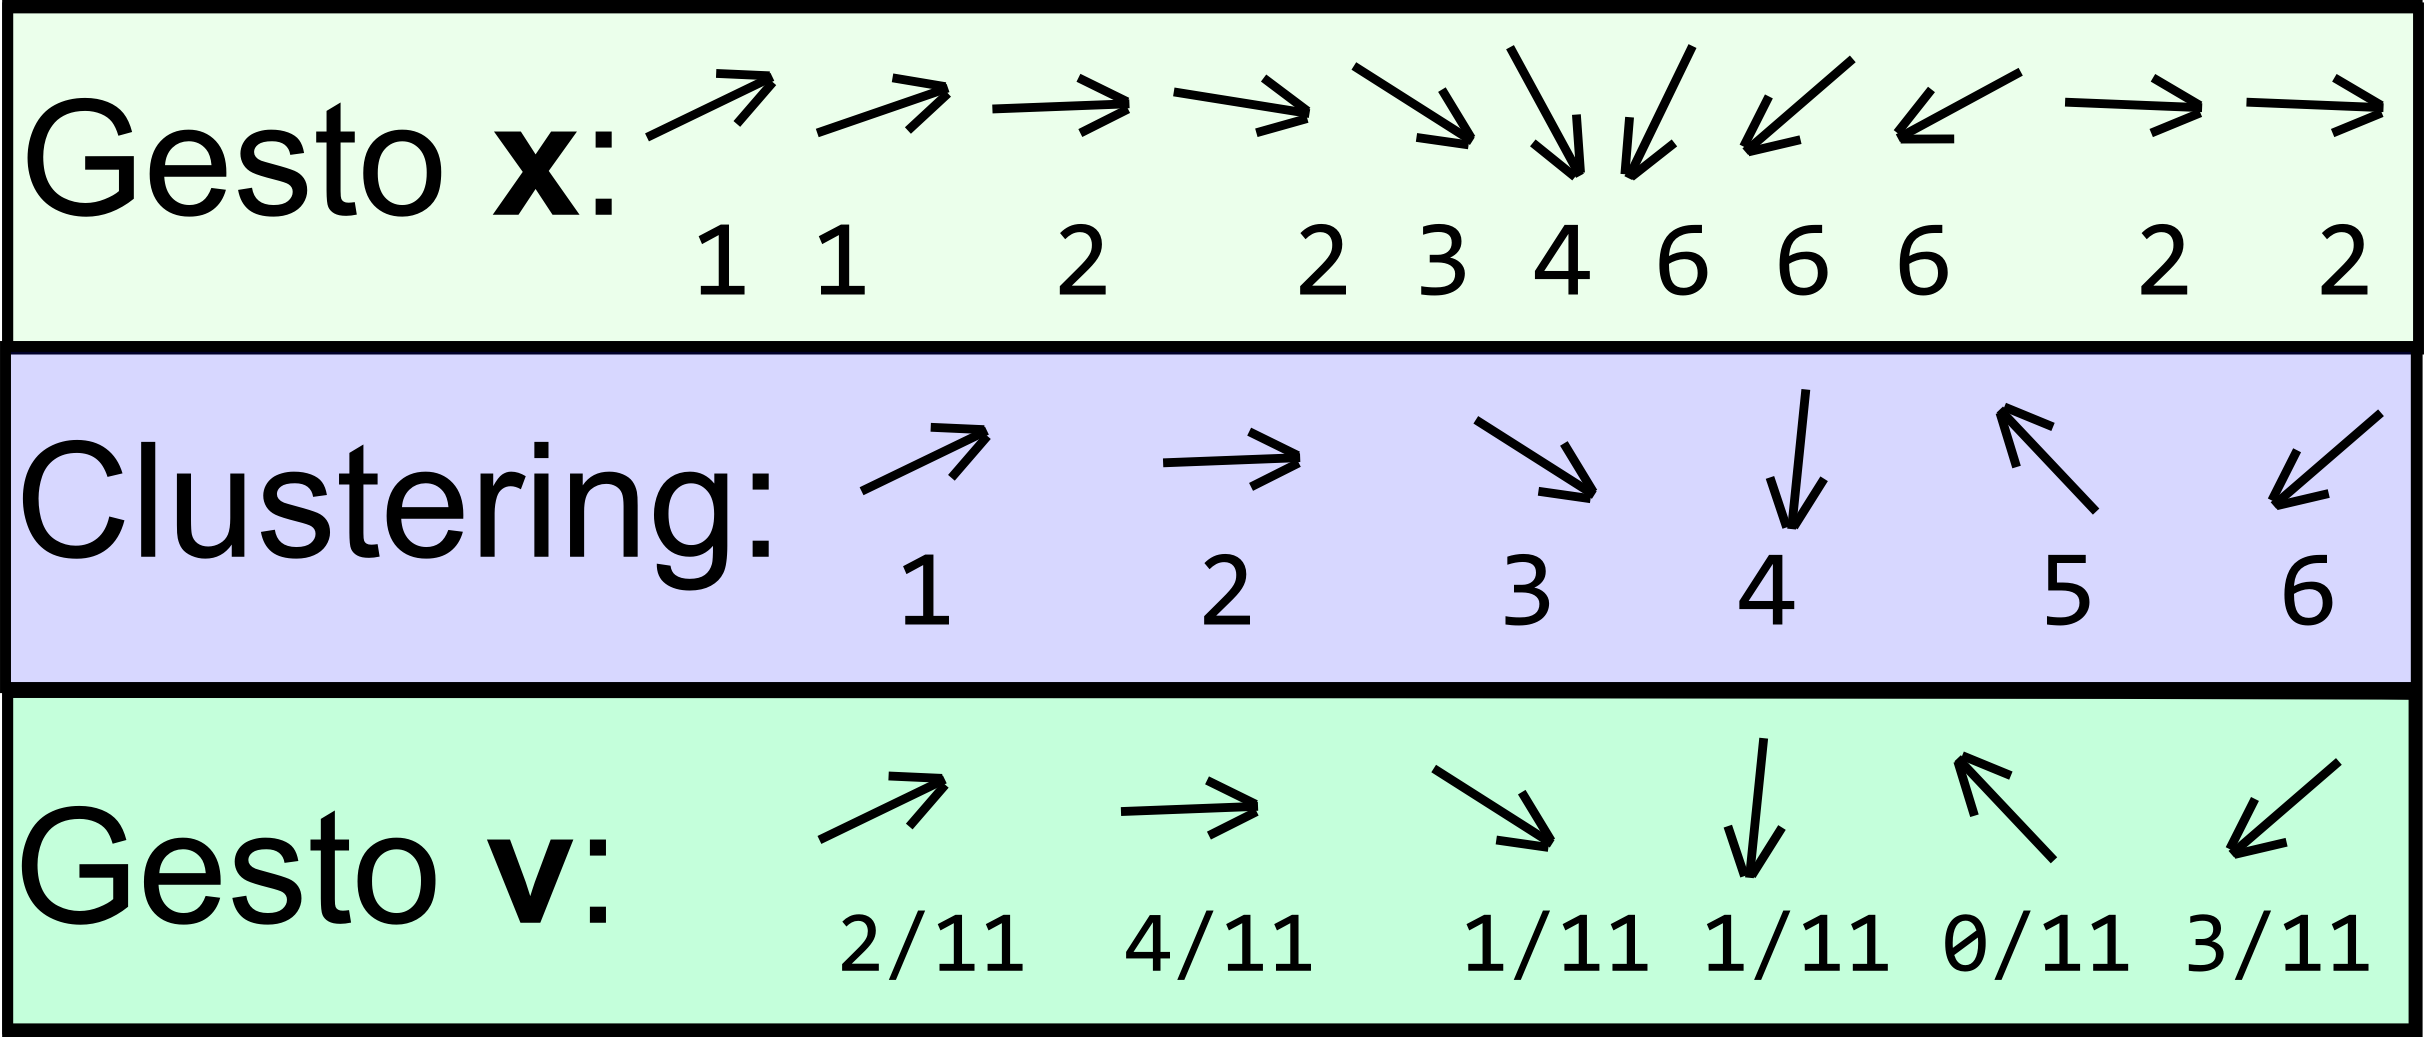
\includegraphics[width=\textwidth]{cnc/codificacion3}
\blockitemize{El CNC genera una codificación de tamaño constante}{
  \item Tamaño del gesto codificado = $h$ = cantidad de neuronas de la capa 2
}
\end{myframe}
